\section{Algorithme \'Evolutionnaire}

La première partie du sujet consistait à retrouver trois valeurs influençant l'orbite de la Terre autour du Soleil : la masse du Soleil, la masse de la Terre et la vitesse de la Terre à la périhélie en utilisant les algorithme évolutionnaires présents dans EASEA.\\
Pour cela nous avons procédé en trois étapes distinctes car la nméthode d'échantillonnage ne permet pas de retrouver les trois quantités simultanément. En effet, il n'est pas possible de retrouver la masse de la Terre et la masse du Soleil en une seule expérience car elles sont uniquement présentes dans un produit dans la formule de Newton. Il existe donc une multitude de couples de valeurs menant au même résultat.\\
La première étape consiste à effectuer un échantillonnage avec les valeurs réelles afin d'obtenir une liste de coordonnées polaires de la Terre dans le référentiel Héliocentrique.\\
Le génome de chaque individu correspond à la quantité à retrouver qui est initialisée à une valeur de l'ordre de grandeur attendu.\\
D'une génération à l'autre, un individu fils correspond à la moyenne de ses deux parents et chaque individu peut muter avec une certaine probabilité. Cette mutation corrrespond à une augmentation ou une diminution d'un certain pourcentage de sa valeur.\\
Afin de calculer le score, on procède à un nouvel échantillonnage de la position de la Terre dans le référentiel Héliocentrique avec la valeur trouvée. Dans le cas de la vitesse de la Terre à la périhélie, la vitesse trouvée est utilisée comme vitesse initiale.\\
Le score correspond à la somme des distances entre les points des deux trajectoires ainsi obtenues. Ainsi le résultat du programme ne dépend pas directement de la valeur à trouver mais d'échantillons qui auraient pu être observés sans connaitre la quantité.\\
Nous utilisons de l'élitisme faible, c'est à dire que le meilleur individu de la population globale (parents et enfants) est garan,ti d'être conservé dans la prochaine génération.

\subsection{Masse du Soleil}

\begin{wrapfigure}{r}{0.5\textwidth}
    \center
    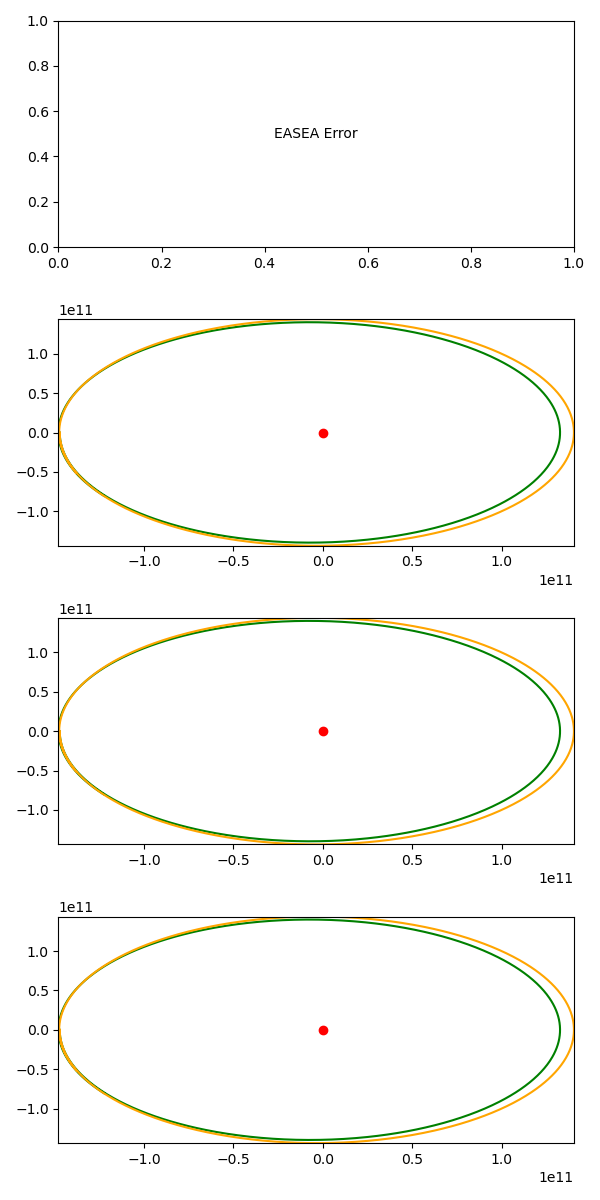
\includegraphics[width=0.5\linewidth,scale=.3]{img/sun_mass.png}
    \caption{Earth trajectories depending of the mass of the Sun}
\end{wrapfigure}
Ceci est du texte !!

\subsection{Masse de la Terre}

\subsection{Vitesse de la Terre à la Périhélie}

